\documentclass[tikz, border=10pt]{standalone}
\usetikzlibrary{angles, quotes, calc}

\begin{document}
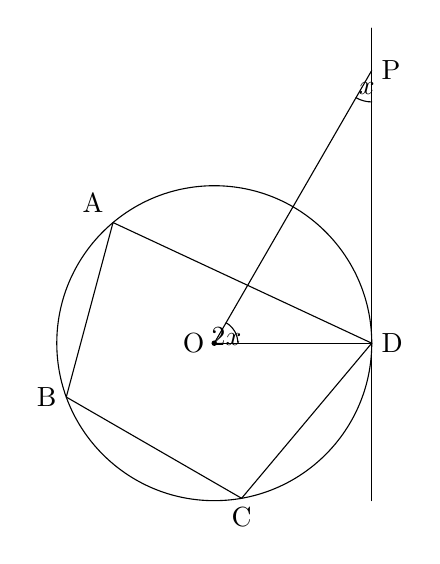
\begin{tikzpicture}[scale=2, line join=round, line cap=round]
    % ১. মূলবিন্দু ও বৃত্তের স্থানাঙ্ক (Center and Circle)
    \coordinate (O) at (0,0);
    \draw (O) circle (1);
    
    % ২. বিন্দু নির্ধারণ (Points)
    \coordinate (D) at (1,0); % স্পর্শবিন্দু
    \coordinate (P) at (1, 1.732); % স্পর্শকের ওপর বিন্দু (tan 60 = 1.732)
    
    % বৃত্তস্থ চতুর্ভুজের বিন্দুসমূহ (Quadrilateral ABCD)
    \coordinate (A) at (130:1);
    \coordinate (B) at (200:1);
    \coordinate (C) at (280:1);

    % ৩. রেখা অঙ্কন (Drawing Lines)
    \draw (A) -- (B) -- (C) -- (D) -- (A); % চতুর্ভুজ ABCD
    \draw (O) -- (D); % ব্যাসার্ধ OD
    \draw (O) -- (P); % কেন্দ্র থেকে P পর্যন্ত রেখা
    \draw (1, -1) -- (1, 2); % স্পর্শক রেখা DP

    % ৪. কোণ নির্দেশক (Angles)
    % কোণ x (at P)
    \pic [draw, angle radius=0.4cm, "$x$"] {angle = O--P--D};
    
    % কোণ 2x (at O)
    \pic [draw, angle radius=0.3cm, "$2x$"] {angle = D--O--P};

    % ৫. লেবেল (Labels)
    \node[left] at (O) {O};
    \node[above left] at (A) {A};
    \node[left] at (B) {B};
    \node[below] at (C) {C};
    \node[right] at (D) {D};
    \node[right] at (P) {P};

    % কেন্দ্রের বিন্দু
    \fill (O) circle (0.5pt);
\end{tikzpicture}
\end{document}